\section{Gewichtsmatrizen\label{gewichtsmatrizenSection}}
In diesem Abschnitt werden verschiedene Gewichtsmatrizen vorgestellt und wie diese erzeugt wurden. Wir haben uns zunächst auf die Erzeugung mit der Gauß-Verteilung konzentriert. Für spätere Anpassungen oder Versuche wurden weitere Funktionen implementiert, wie zum Beispiel die Rayleigh-Funktion oder der Tangenshyperbolicus, jedoch nicht ausgewertet.

Zunächst soll erläutert werden, wie die Gewichtsmatrizen grob erstellt wurden. Dafür werden im Abschnitt \ref{eGeW} 3 Beispiele mit jeweils einem Slope, beziehungsweise einer Steigung, von 75 gezeigt. Es soll außerdem verdeutlicht werden, dass es sich immer nur um einen Gauß in x- und y-Richtung handelt. Des Weiteren ist das Endergebnis immer zwischen -1 und 1 definiert, obwohl auch dies variabel eingestellt werden kann. Jedoch kann somit später der Ergebnisbereich einfacher skaliert werden. Die vollständige Erzeugung der Gewichtsmatrizen für diese Beipiele ist im Appendix \ref{GetGaussWeights} aufgeführt. In den anderen Unterabschnitten sind für jede Art der Gewichtsmatrizen unterschiedliche Steigungen eingestellt.

\newpage
\subsection{Erzeugung der Gewichtsmatrizen \label{eGeW}} 
\begin{figure}[hbt]
	\centering
	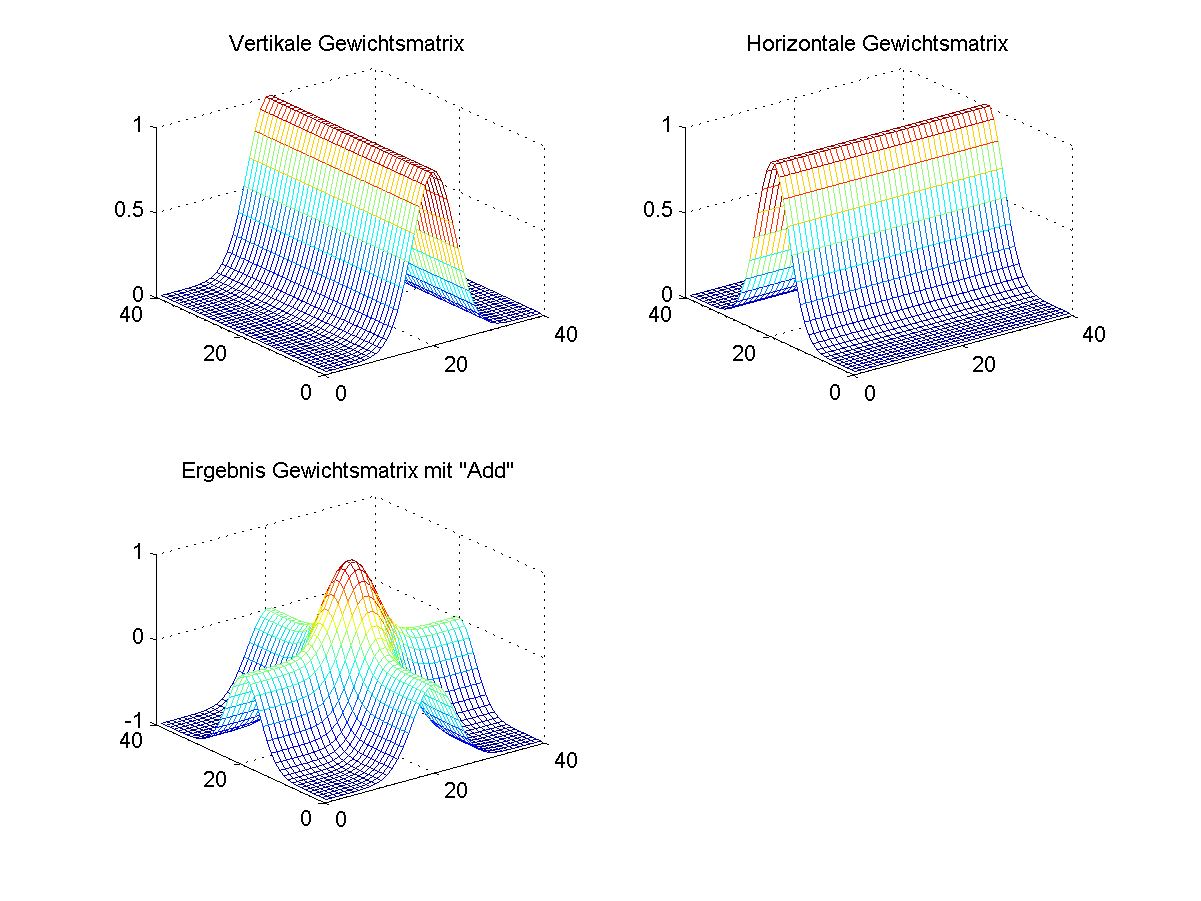
\includegraphics[trim=70 191 42 152, clip, width=0.95\linewidth]{./Bilder/Auswertung/GewichtmatrixEinzelschritte/Endergebnis_Gewichtsmatrix_Slope_75_Type_Add}
	\caption{Additive Überlagerung mit Slope von 75}
	\label{Add75}
\end{figure}
In Abbildung \ref{Add75} wurde der 3D-Gauß in x- und y-Richtung additiv Überlagert, mit 2 multipliziert und am Ende um 1 heruntergesetzt. Siehe Listing \ref{code:Add75}.
\lstinputlisting[language=MATLAB, caption=Auszug GetGaussWeights: Additive Überlagerung \ref{GetGaussWeights}, numbers=left, firstline=74, lastline=78, firstnumber=74]{../Tool/GetGaussWeights.m} \label{code:Add75}

\newpage
\begin{figure}[hbt]
	\centering
	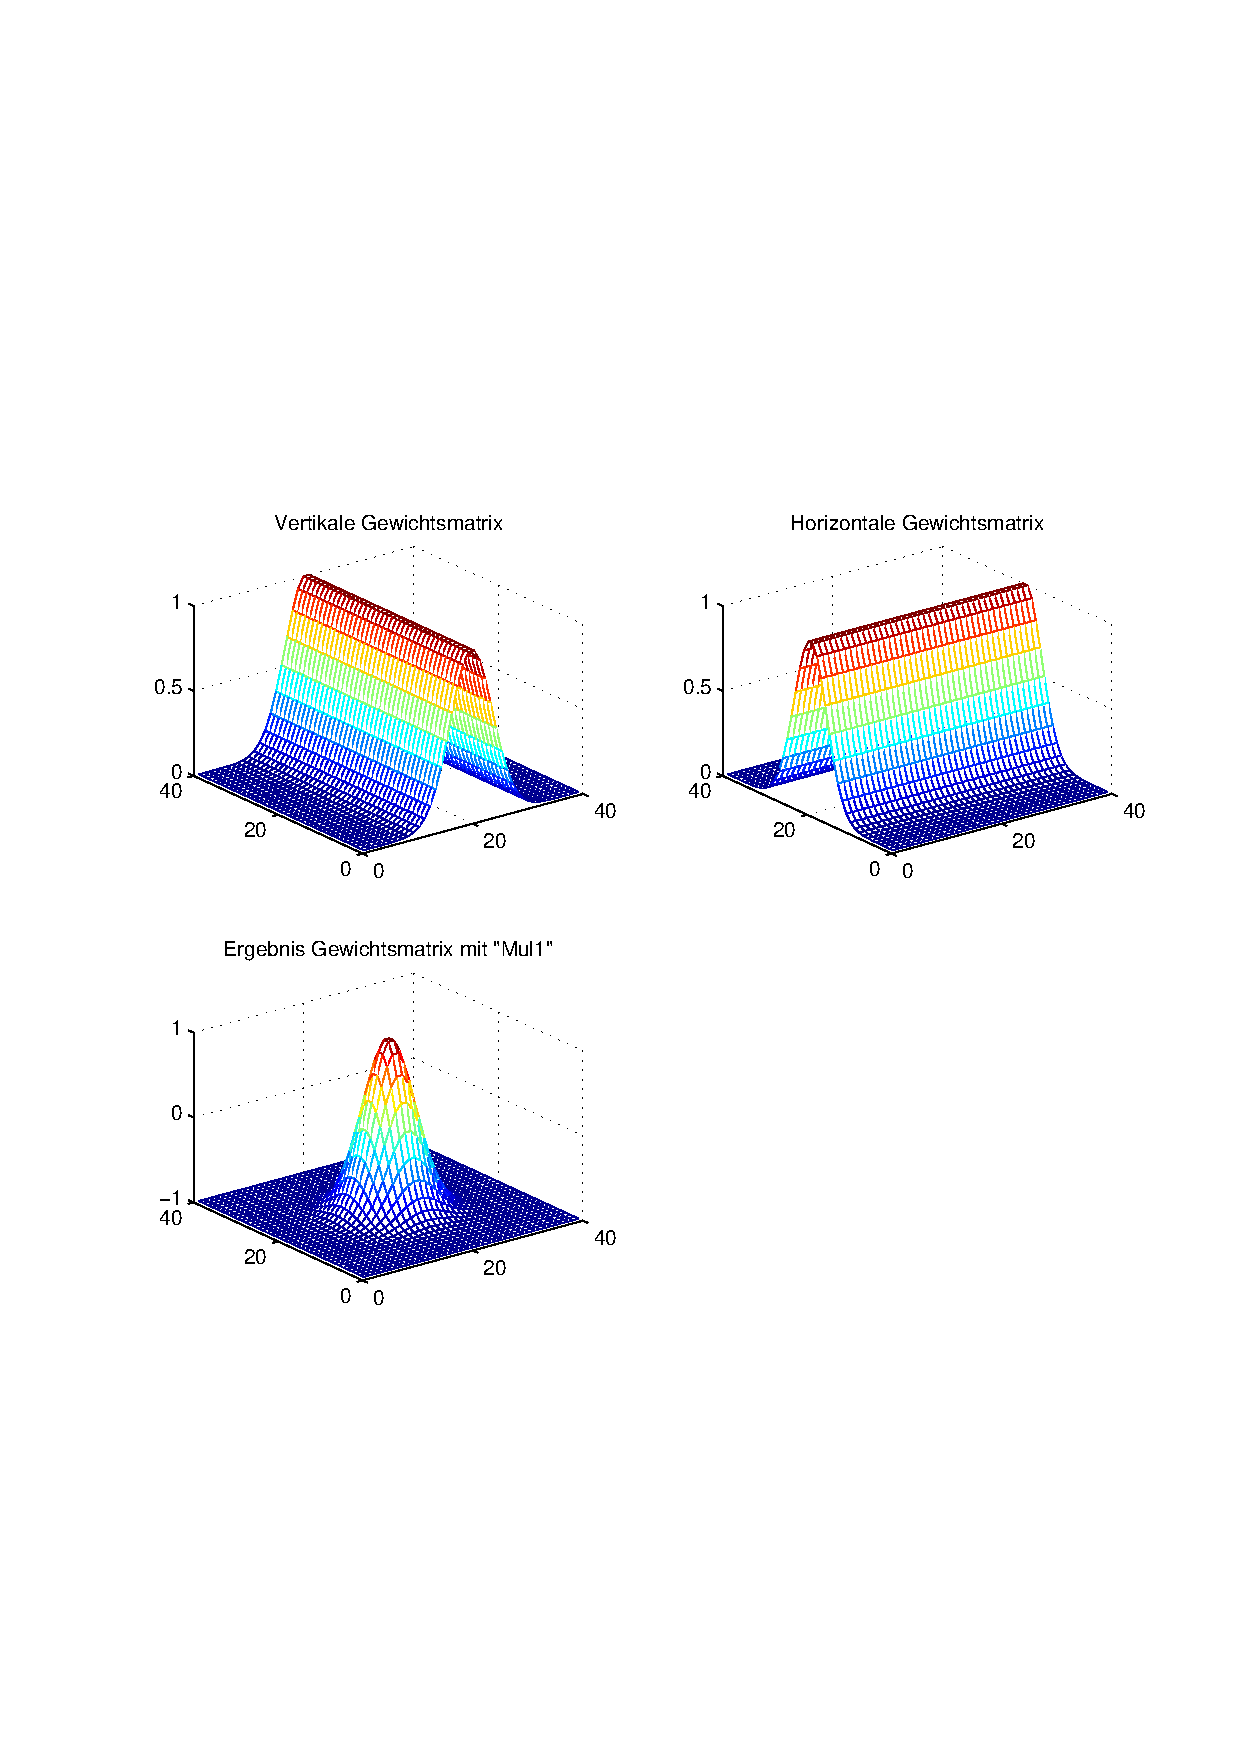
\includegraphics[trim=70 191 42 152, clip, width=0.95\linewidth]{./Bilder/Auswertung/GewichtmatrixEinzelschritte/Endergebnis_Gewichtsmatrix_Slope_75_Type_Mul1}
	\caption{Multiplikative Überlagerung Typ 1 mit Slope von 75}
	\label{Mul175}
\end{figure}

In Abbildung \ref{Mul175} wurde der 3D-Gauß in x-Richtung  mit dem 3D Gauß in y-Richtung multiplikativ Überlagert, mit 2 multipliziert und um 1 heruntergesetzt. Siehe Listing \ref{code:Mul175}.

\lstinputlisting[language=MATLAB, caption=Auszug GetGaussWeights: Multiplikative Überlagerung Typ 1 \ref{GetGaussWeights}, label=code:Mul175, numbers=left, firstline=62, lastline=66, firstnumber=62]{../Tool/GetGaussWeights.m}

\newpage
\begin{figure}[hbt]
	\centering
	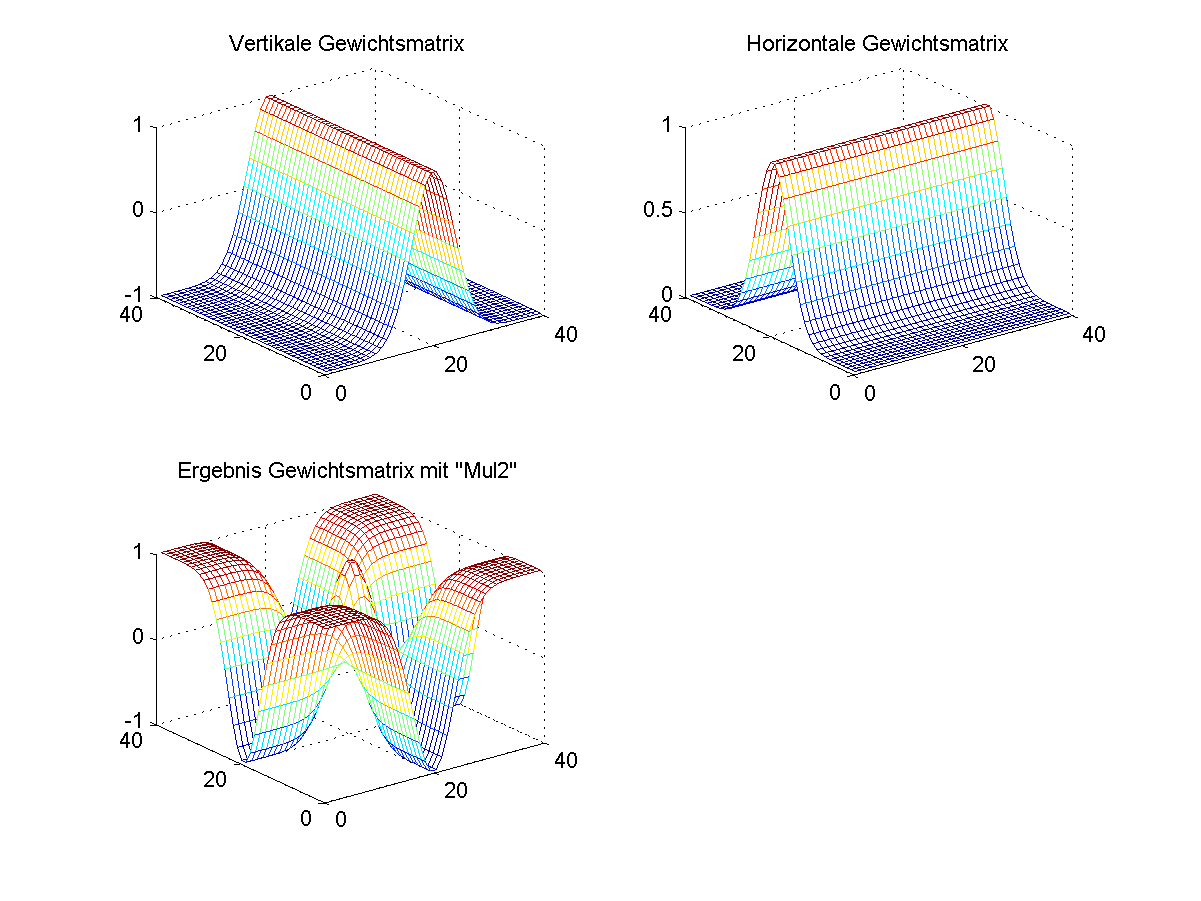
\includegraphics[trim=70 191 42 152, clip, width=0.95\linewidth]{./Bilder/Auswertung/GewichtmatrixEinzelschritte/Endergebnis_Gewichtsmatrix_Slope_75_Type_Mul2}
	\caption{Multiplikative Überlagerung Typ 2 mit Slope von 75}
	\label{Mul275}
\end{figure}

In Abbildung \ref{Mul275} wurde der 3D-Gauß in y-Richtung erst einmal zwischen -1 und 1 skaliert. Anschließend wird der 3D-Gauß in x-Richtung ebenfalls zwischen -1 und 1 skaliert. Am Ende werden beide multiplikativ überlagert. Siehe auch das Listing \ref{code:Mul275}.

\lstinputlisting[language=MATLAB, caption=Auszug GetGaussWeights: Multiplikative Überlagerung Typ 2 \ref{GetGaussWeights}, label=code:Mul275, numbers=left, firstline=67, lastline=73, firstnumber=67]{../Tool/GetGaussWeights.m}

\newpage
\subsection{Additive Überlagerung}
Ergebnisse der Additiven Überlagerung mit unterschiedlichen Slope-Werten.
\begin{figure}[hbt]
	\begin{minipage}{0.48\textwidth}
		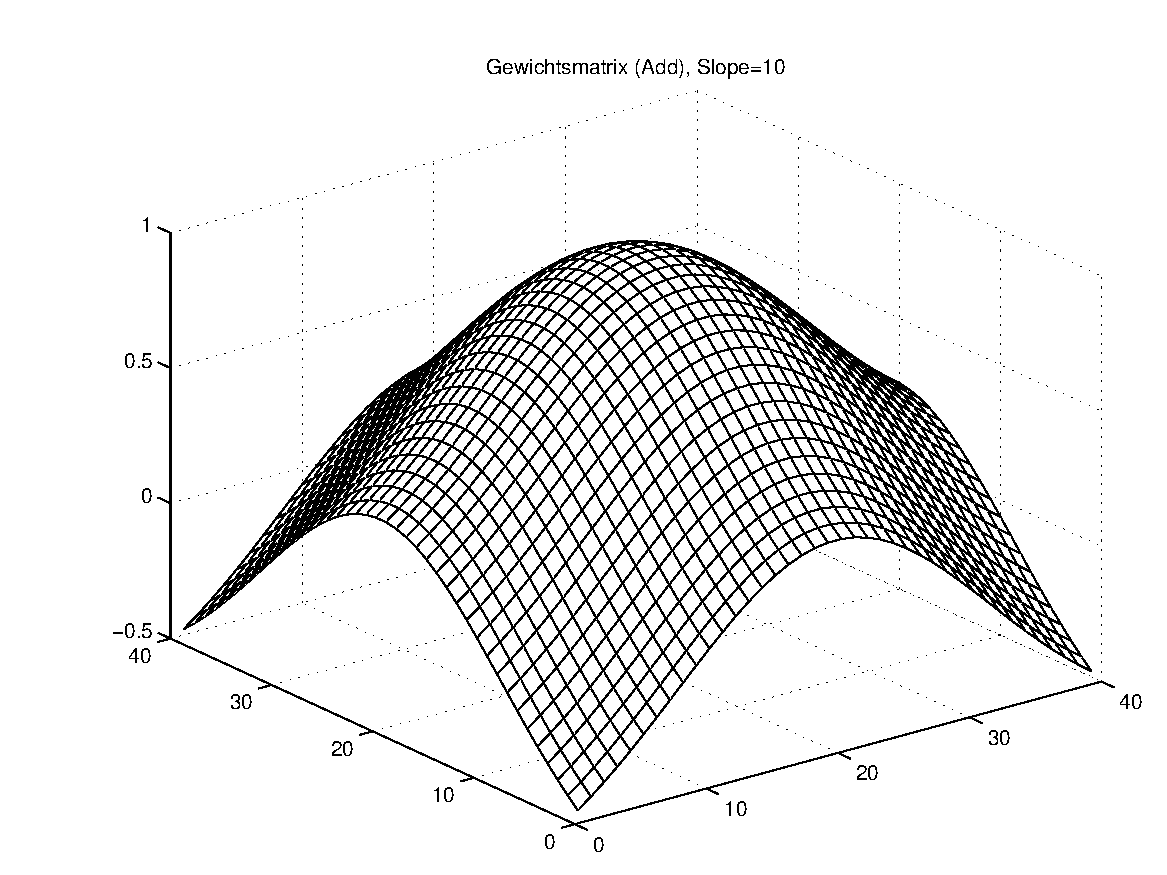
\includegraphics[trim=70 200 32 242, clip, width=\textwidth]{./Bilder/Auswertung/Gewichtsmatrix/Gewichtsmatrix_Add_Slope_10}
		\caption{Additive mit Slope 10}
		\label{Add10}
	\end{minipage}
	\hfill
	\begin{minipage}{0.48\textwidth}
		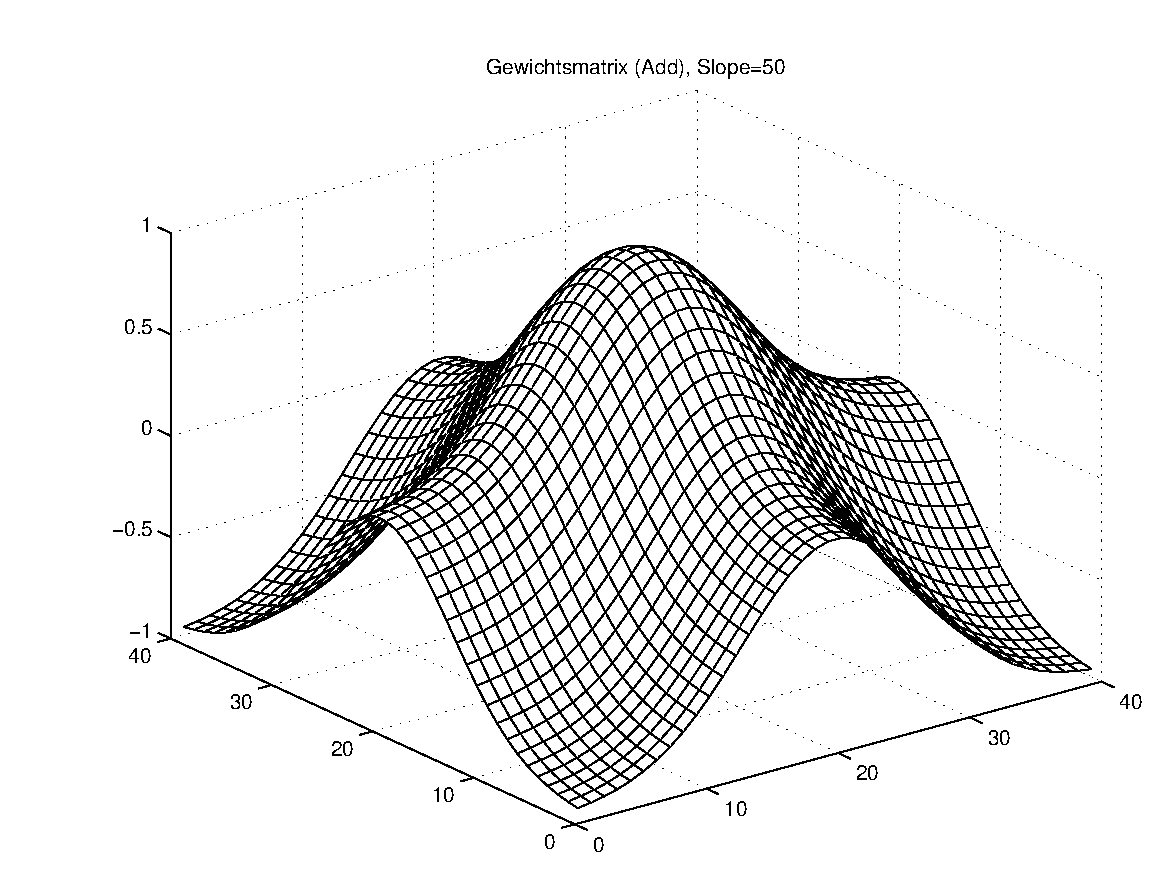
\includegraphics[trim=70 200 32 242, clip, width=\textwidth]{./Bilder/Auswertung/Gewichtsmatrix/Gewichtsmatrix_Add_Slope_50}
		\caption{Additive mit Slope 50}
		\label{Add50}
	\end{minipage}
\end{figure}
\begin{figure}[hbt]
	\centering
	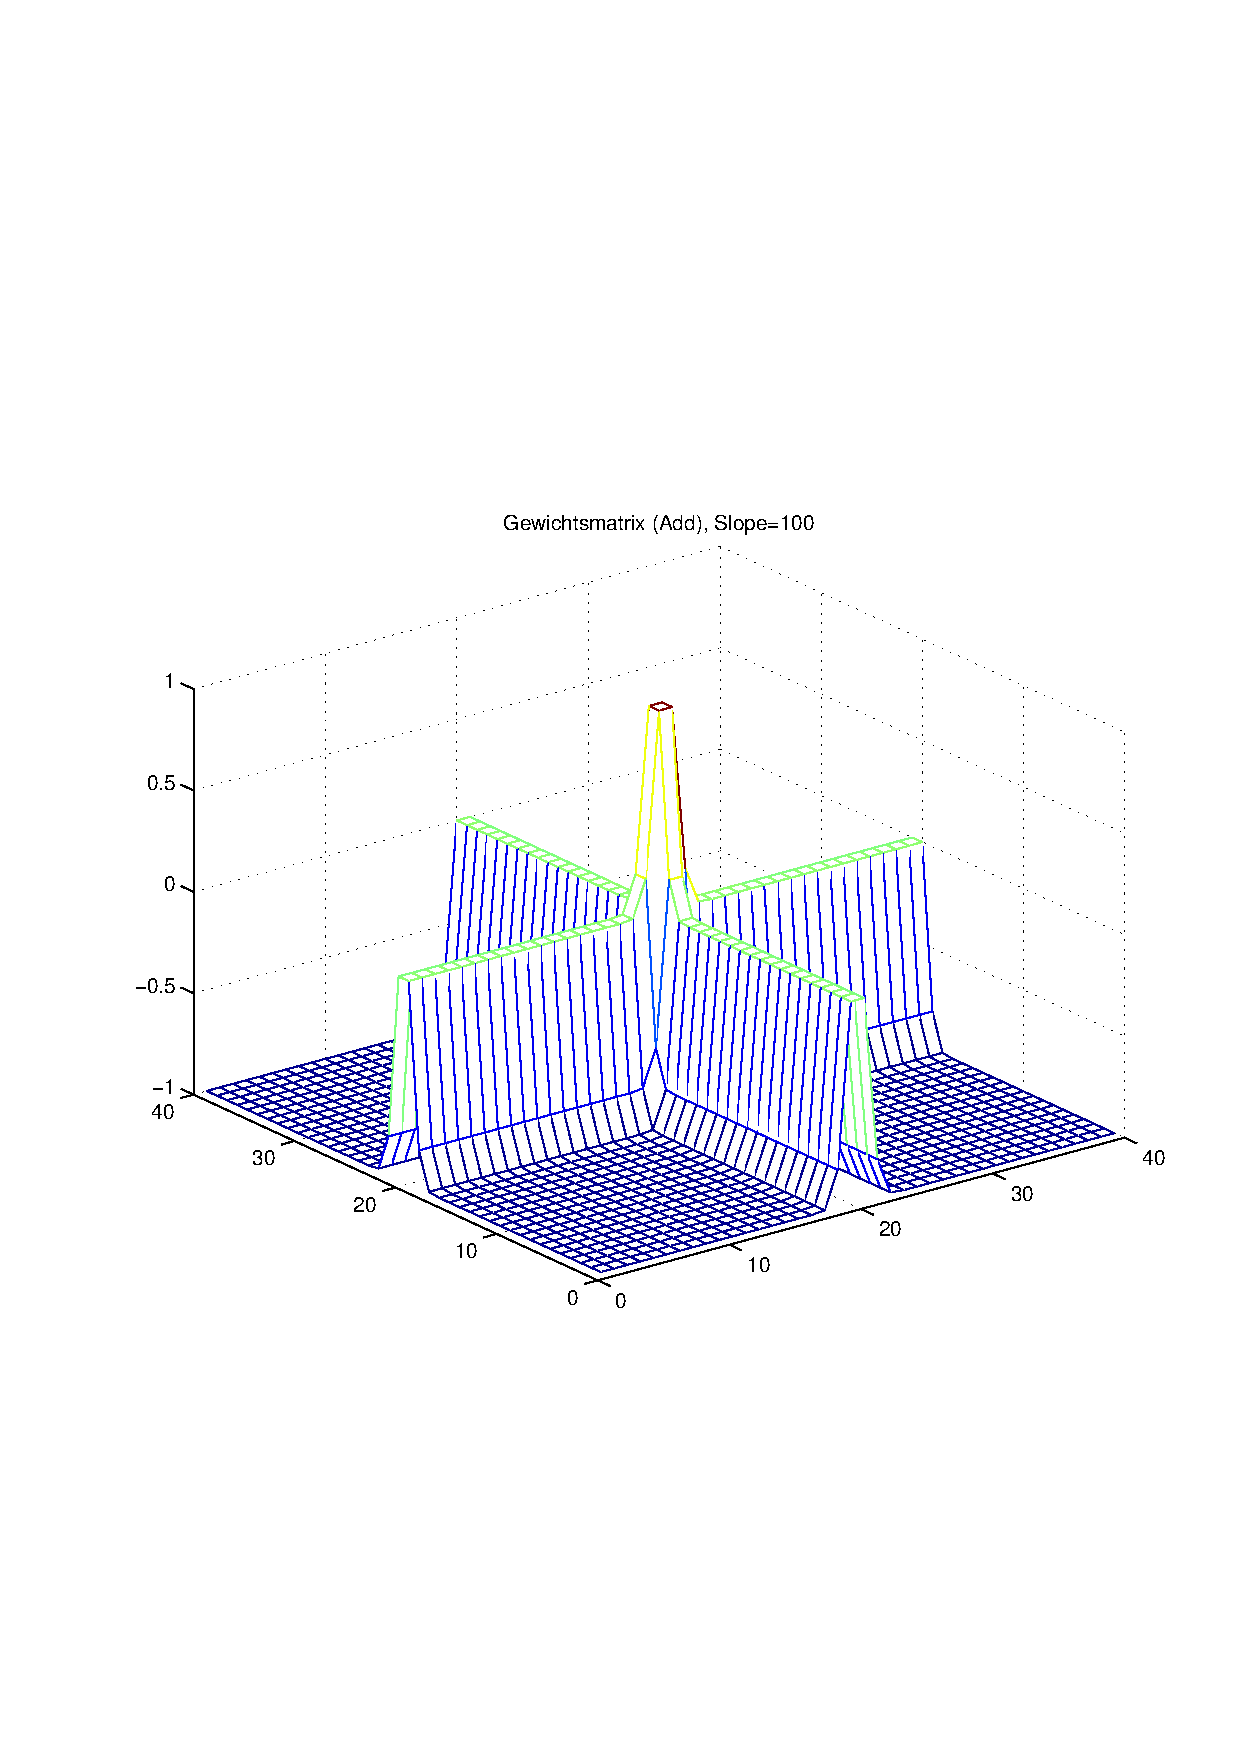
\includegraphics[trim=70 200 32 242, clip, width=0.48\linewidth]{./Bilder/Auswertung/Gewichtsmatrix/Gewichtsmatrix_Add_Slope_100}
	\caption{Additive Überlagerung mit Slope von 100}
	\label{Add100}
\end{figure}

\newpage
\subsection{Multiplikative Überlagerung Typ 1}
Ergebnisse der Multiplikativen Überlagerung Typ 1 mit unterschiedlichen Slope-Werten.
\begin{figure}[hbt]
	\begin{minipage}{0.48\textwidth}
		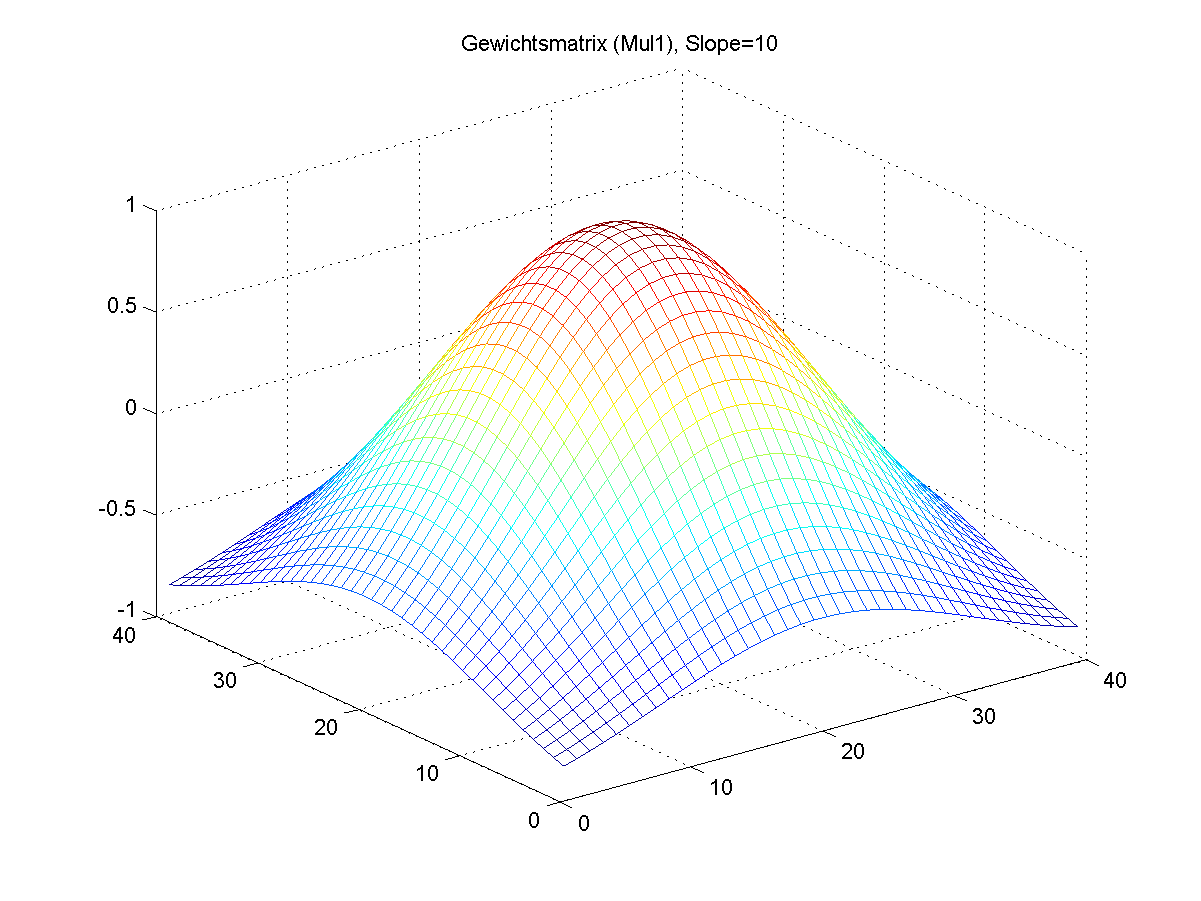
\includegraphics[trim=70 200 32 242, clip, width=\textwidth]{./Bilder/Auswertung/Gewichtsmatrix/Gewichtsmatrix_Mul1_Slope_10}
		\caption{Multi-Typ 1 mit Slope von 10}
		\label{Mul110}
	\end{minipage}
	\hfill
	\begin{minipage}{0.48\textwidth}
		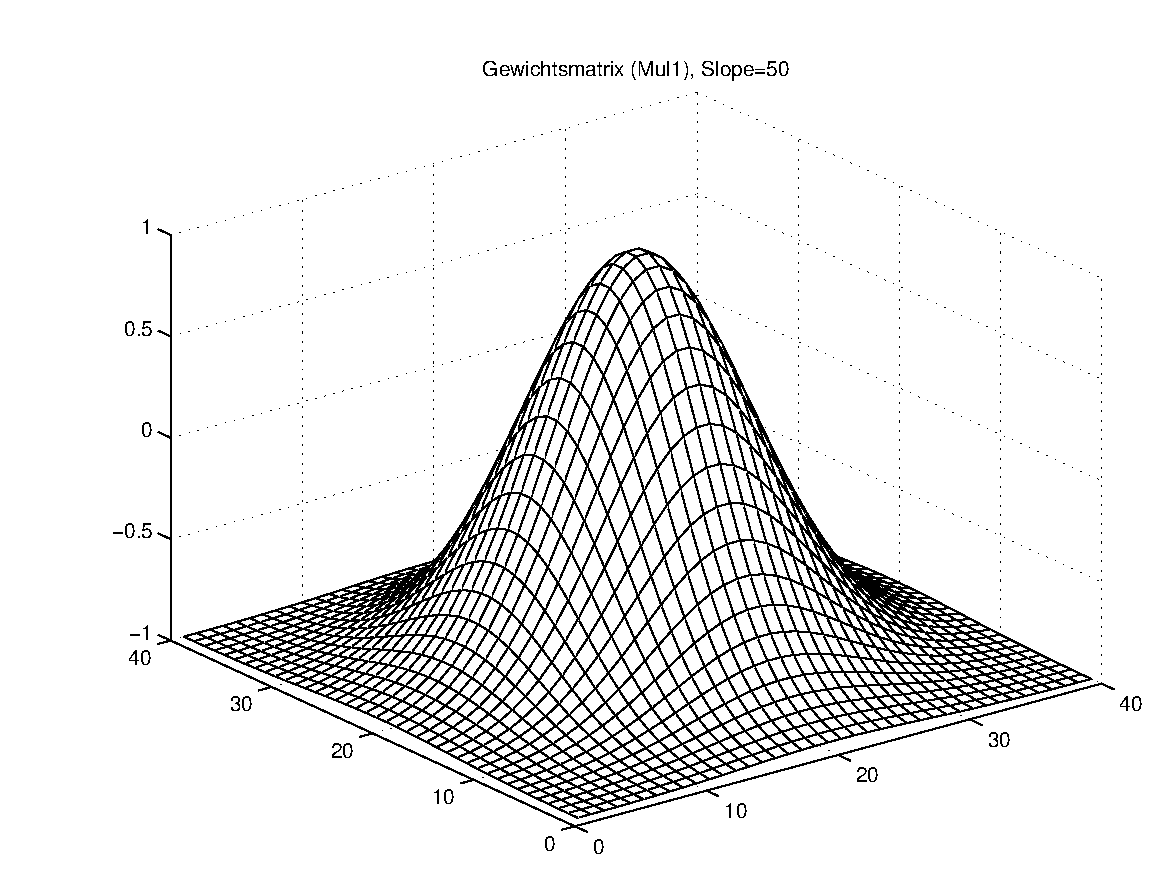
\includegraphics[trim=70 200 32 242, clip, width=\textwidth]{./Bilder/Auswertung/Gewichtsmatrix/Gewichtsmatrix_Mul1_Slope_50}
		\caption{Multi-Typ 1 mit Slope von 50}
		\label{Mul150}
	\end{minipage}
\end{figure}
\begin{figure}[hbt]
	\centering
	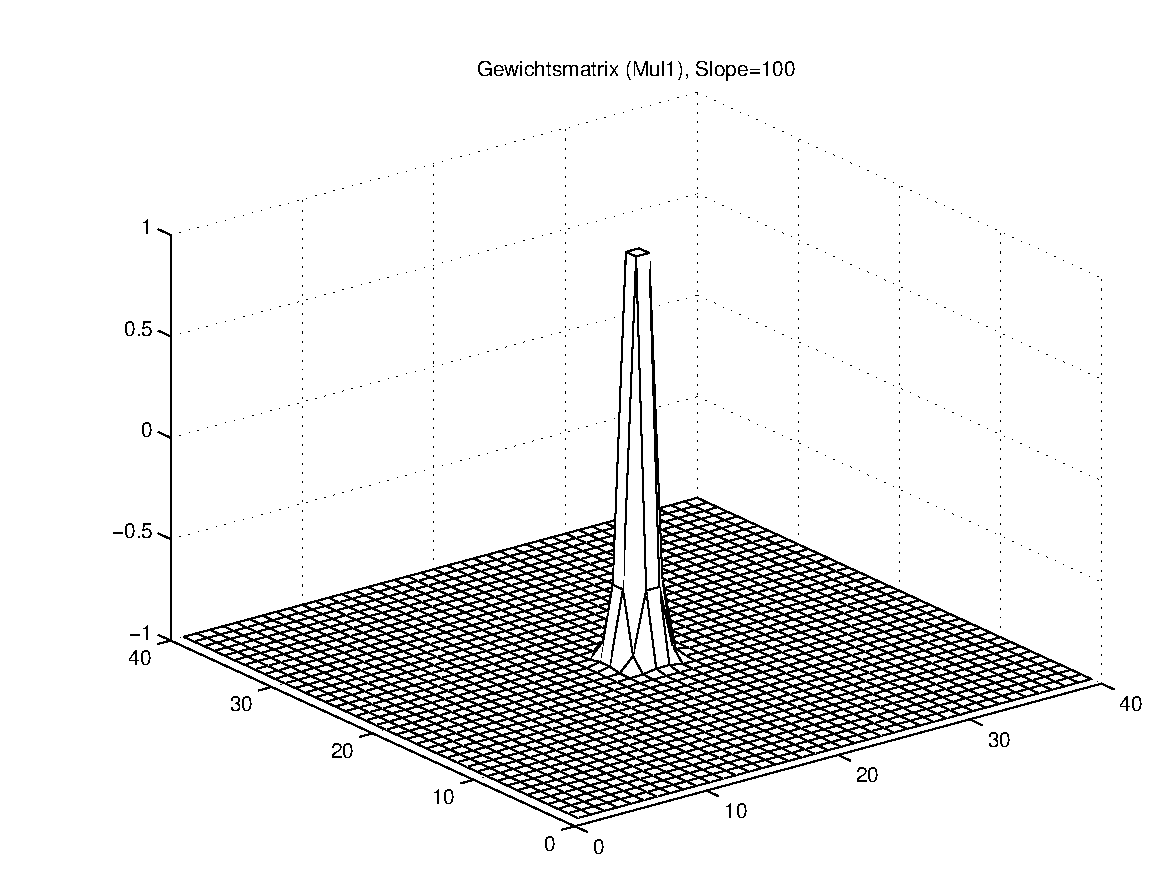
\includegraphics[trim=70 200 32 242, clip, width=0.48\linewidth]{./Bilder/Auswertung/Gewichtsmatrix/Gewichtsmatrix_Mul1_Slope_100}
	\caption{Multiplikative Überlagerung Typ 1 mit Slope von 100}
	\label{Mul1100}
\end{figure}

\newpage
\subsection{Multiplikative Überlagerung Typ 2}
Ergebnisse der Multiplikativen Überlagerung Typ 1 mit unterschiedlichen Slope-Werten.
\begin{figure}[hbt]
	\begin{minipage}{0.48\textwidth}
		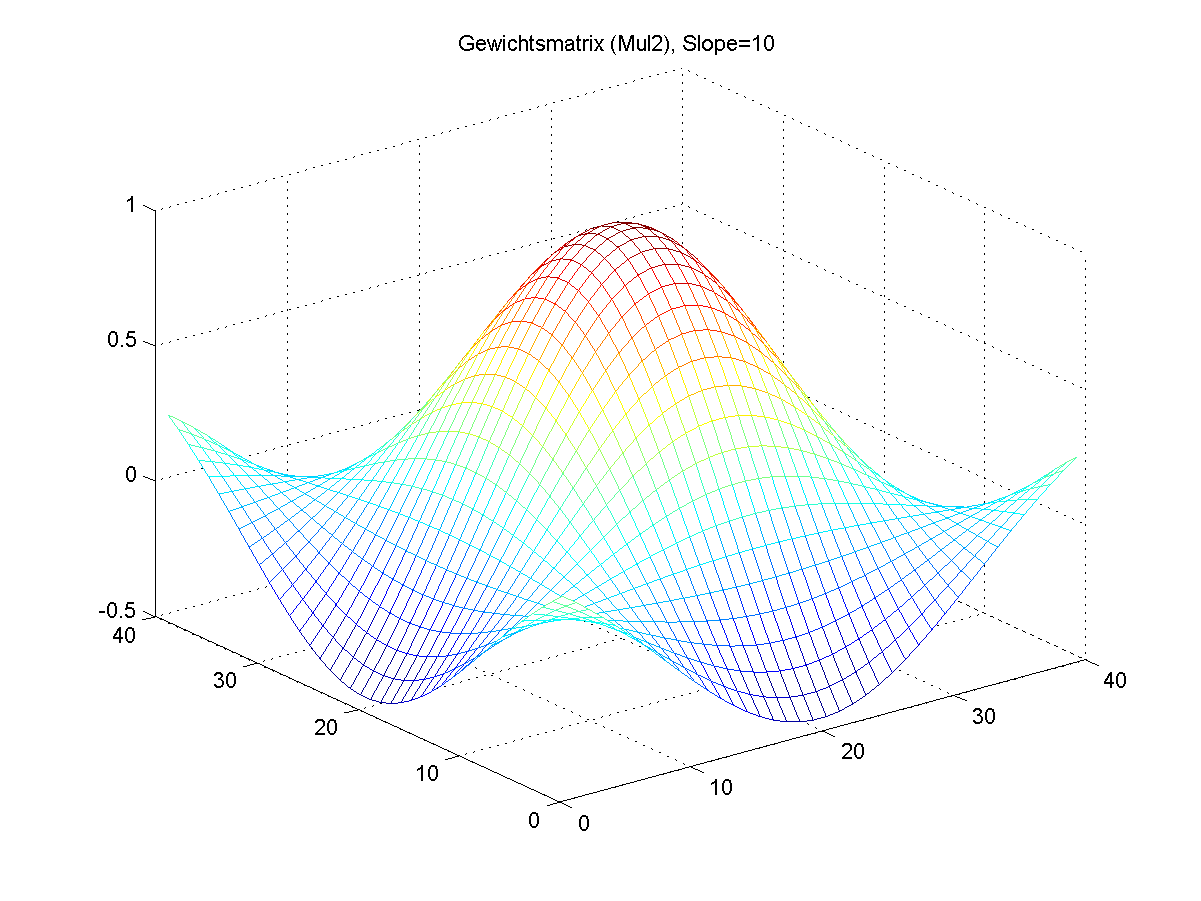
\includegraphics[trim=70 200 32 242, clip, width=\textwidth]{./Bilder/Auswertung/Gewichtsmatrix/Gewichtsmatrix_Mul2_Slope_10}
		\caption{Multi-Typ 2 mit Slope von 10}
		\label{Mul210}
	\end{minipage}
	\hfill
	\begin{minipage}{0.48\textwidth}
		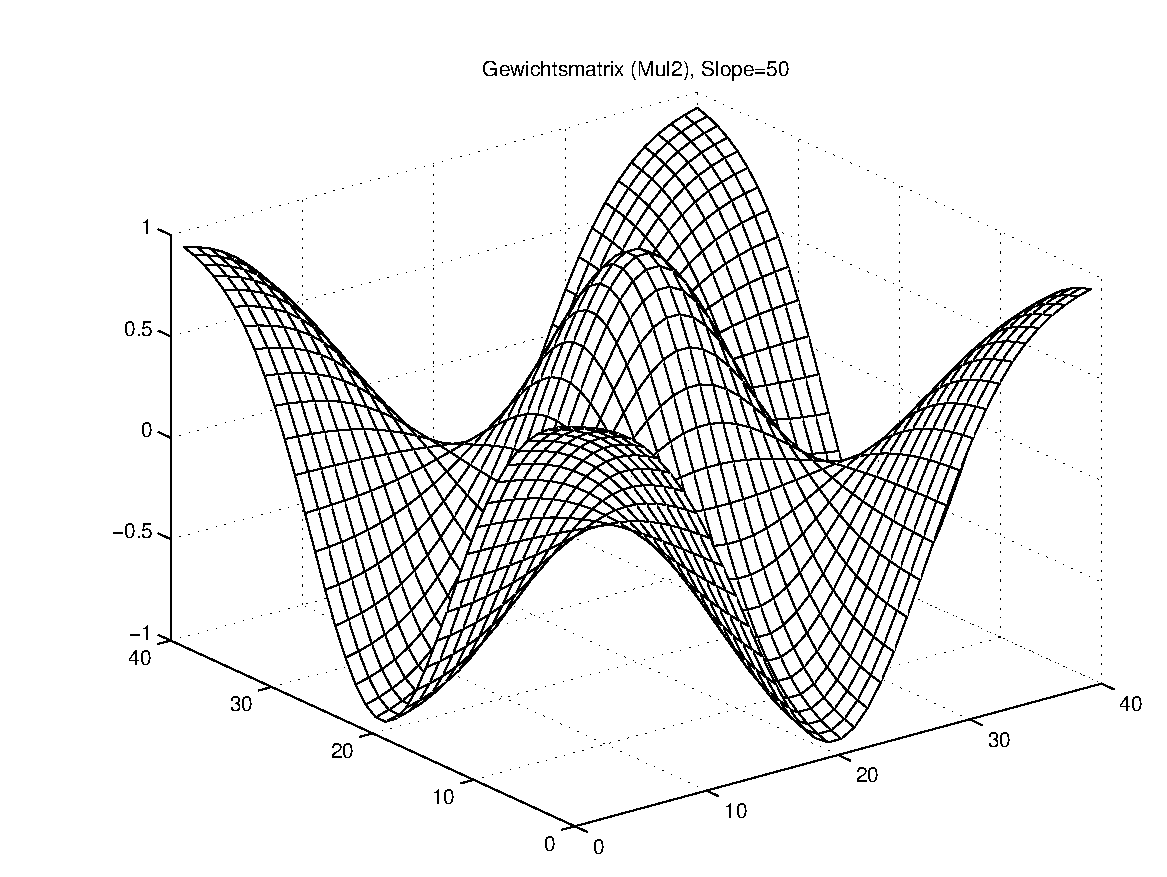
\includegraphics[trim=70 200 32 242, clip, width=\textwidth]{./Bilder/Auswertung/Gewichtsmatrix/Gewichtsmatrix_Mul2_Slope_50}
		\caption{Multi-Typ 2 mit Slope von 50}
		\label{Mul250}
	\end{minipage}
\end{figure}
\begin{figure}[hbt]
	\centering
	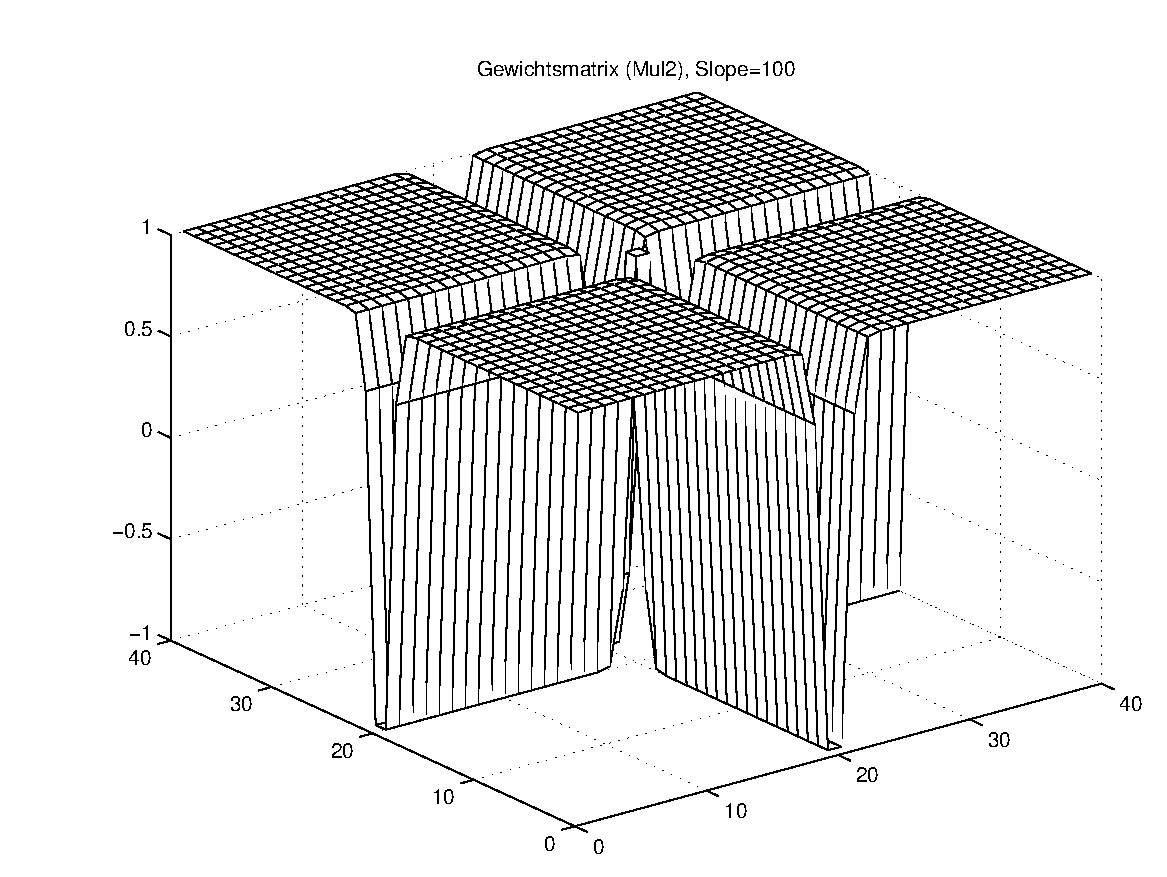
\includegraphics[trim=70 200 32 242, clip, width=0.48\linewidth]{./Bilder/Auswertung/Gewichtsmatrix/Gewichtsmatrix_Mul2_Slope_100}
	\caption{Multiplikative Überlagerung Typ 2 mit Slope von 100}
	\label{Mul2100}
\end{figure}

\newpage
\subsection{Additive und Multiplikative Überlagerung}
Diese Art der Überlagerung entstand als Idee die Überhöhung im Zentrum der Gewichtsmatrix, siehe Abbildung \ref{Add75}, zu vermeiden und zusätzlich die \"Schultern\" auf 1 anzuheben. Hierfür werden die beiden Gauß-Matrizen zunächst additiv überlagert und anschließend wird die multiplikative Überlagerung abgezogen. Siehe Listing \ref{code:AddMul}. Die Beschriftung wurde mit 'AddMul' abgekürzt.
\lstinputlisting[language=MATLAB, caption=Auszug GetGaussWeights: 'AddMul'-Überlagerung \ref{GetGaussWeights}, label=code:AddMul, numbers=left, firstline=79, lastline=89, firstnumber=79]{../Tool/GetGaussWeights.m}
\begin{figure}[hbt]
	\begin{minipage}{0.45\textwidth}
		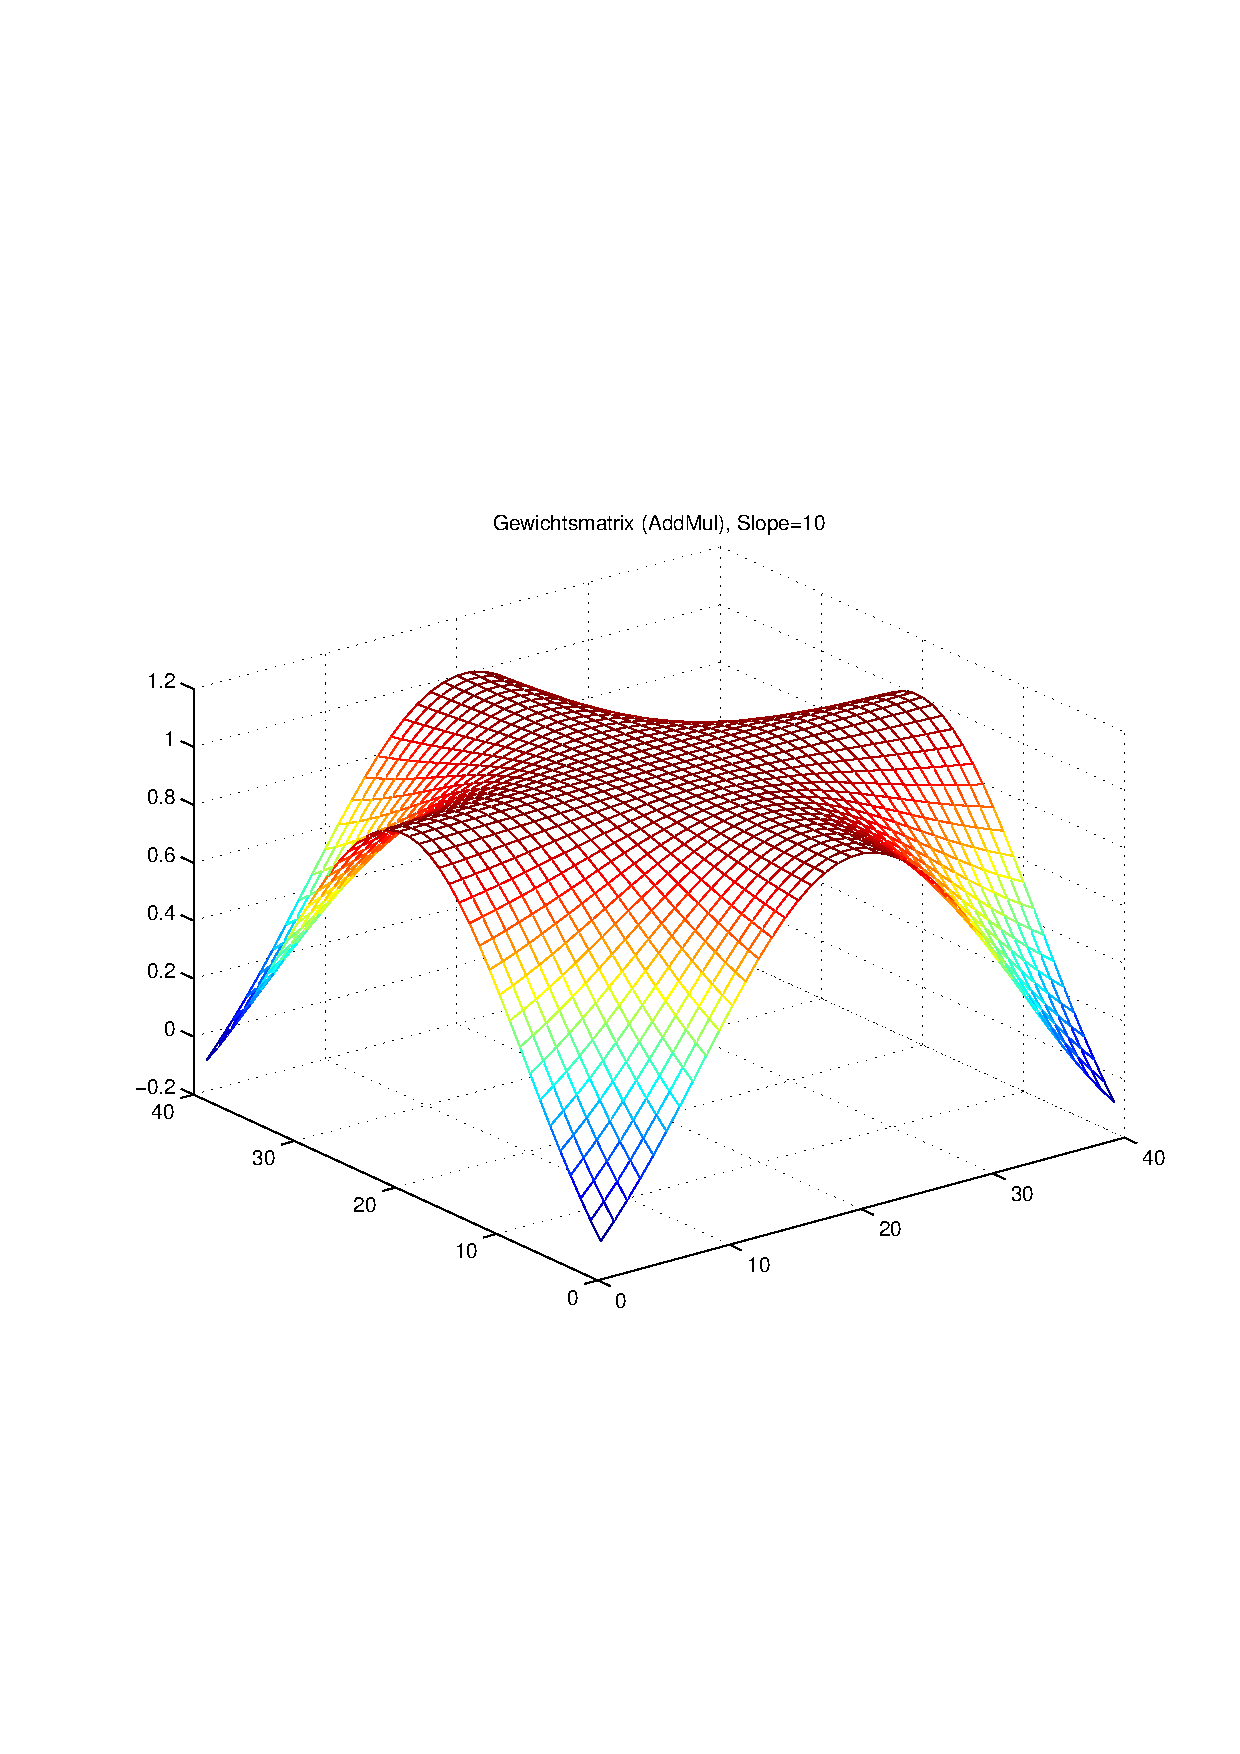
\includegraphics[trim=70 200 32 242, clip, width=\textwidth]{./Bilder/Auswertung/Gewichtsmatrix/Gewichtsmatrix_AddMul_Slope_10}
		\caption{AddMul mit Slope 10}
		\label{AddMul210}
	\end{minipage}
	\hfill
	\begin{minipage}{0.45\textwidth}
		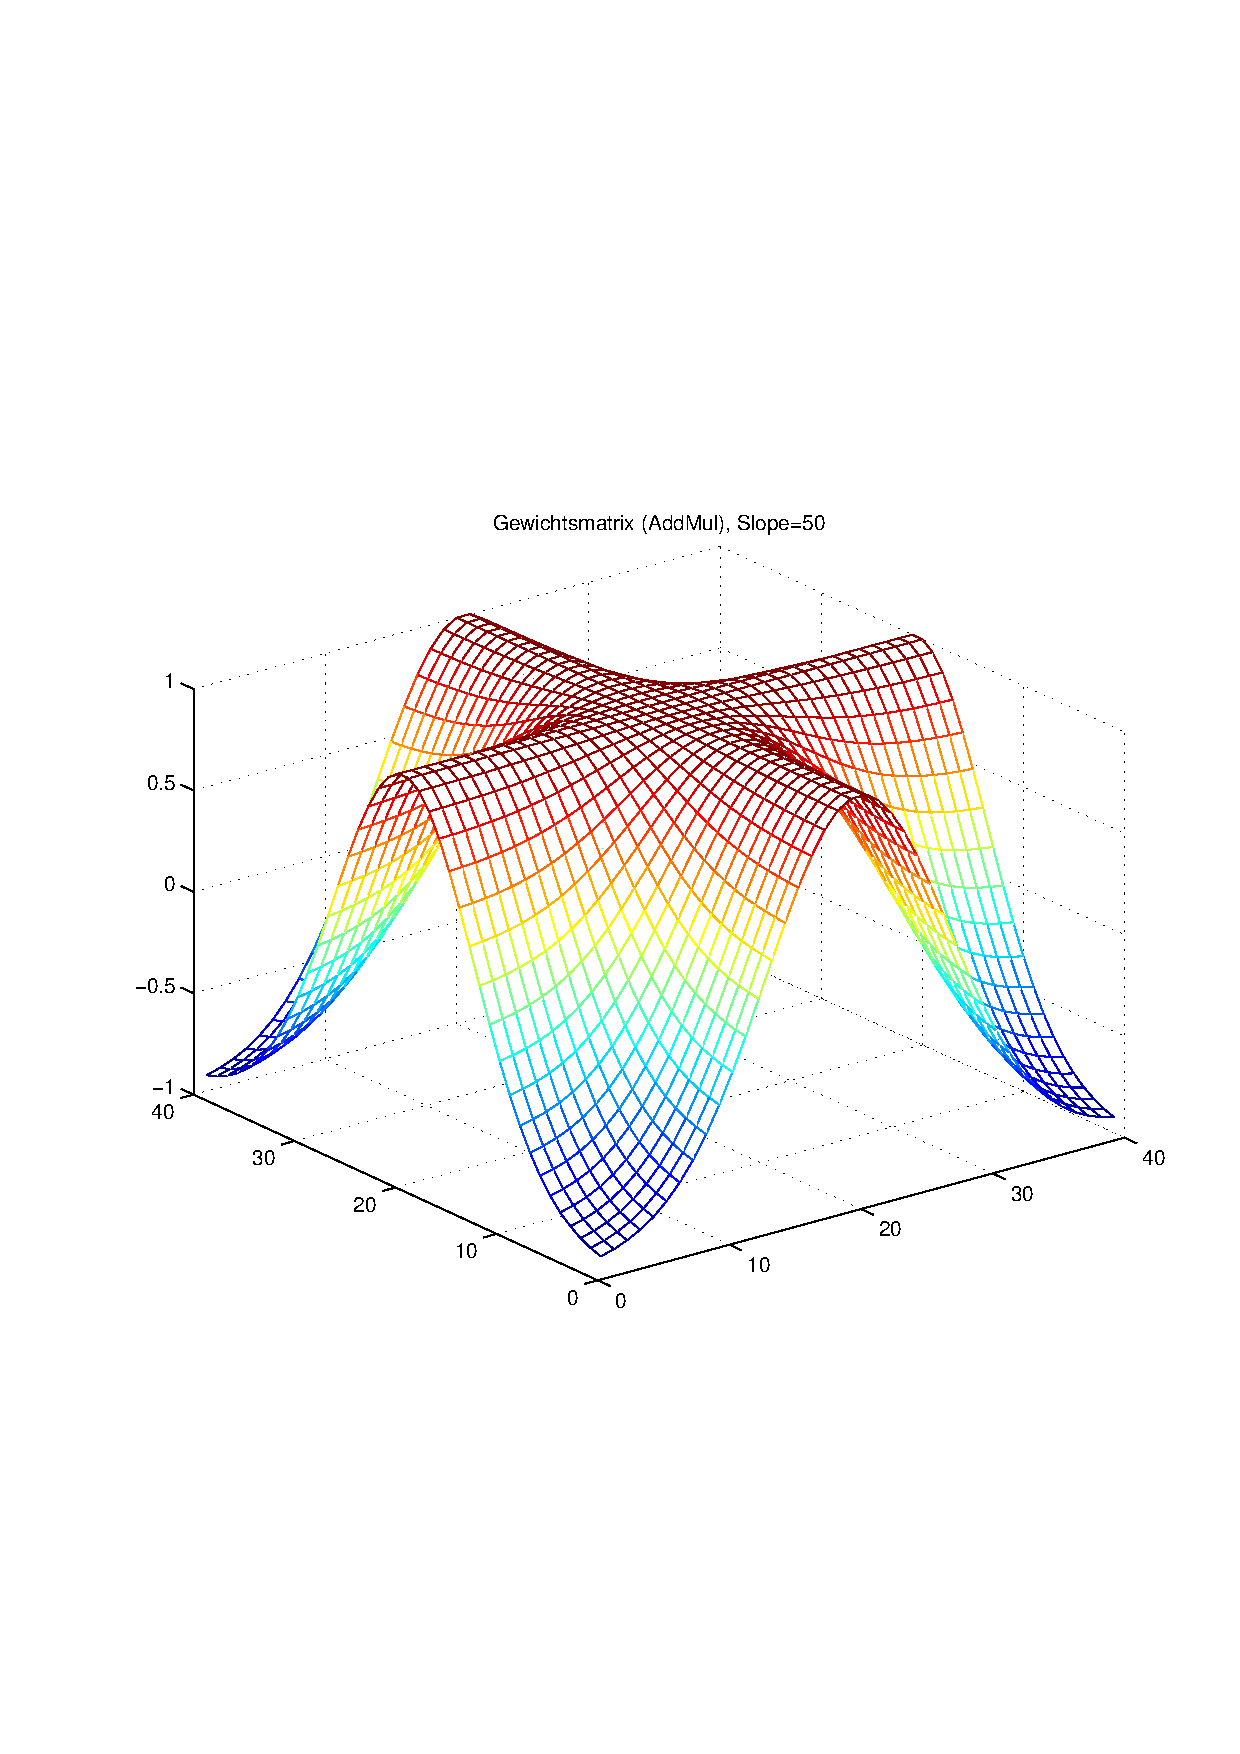
\includegraphics[trim=70 200 32 242, clip, width=\textwidth]{./Bilder/Auswertung/Gewichtsmatrix/Gewichtsmatrix_AddMul_Slope_50}
		\caption{AddMul mit Slope 50}
		\label{AddMul50}
	\end{minipage}
\end{figure}
\begin{figure}[hbt]
	\centering
	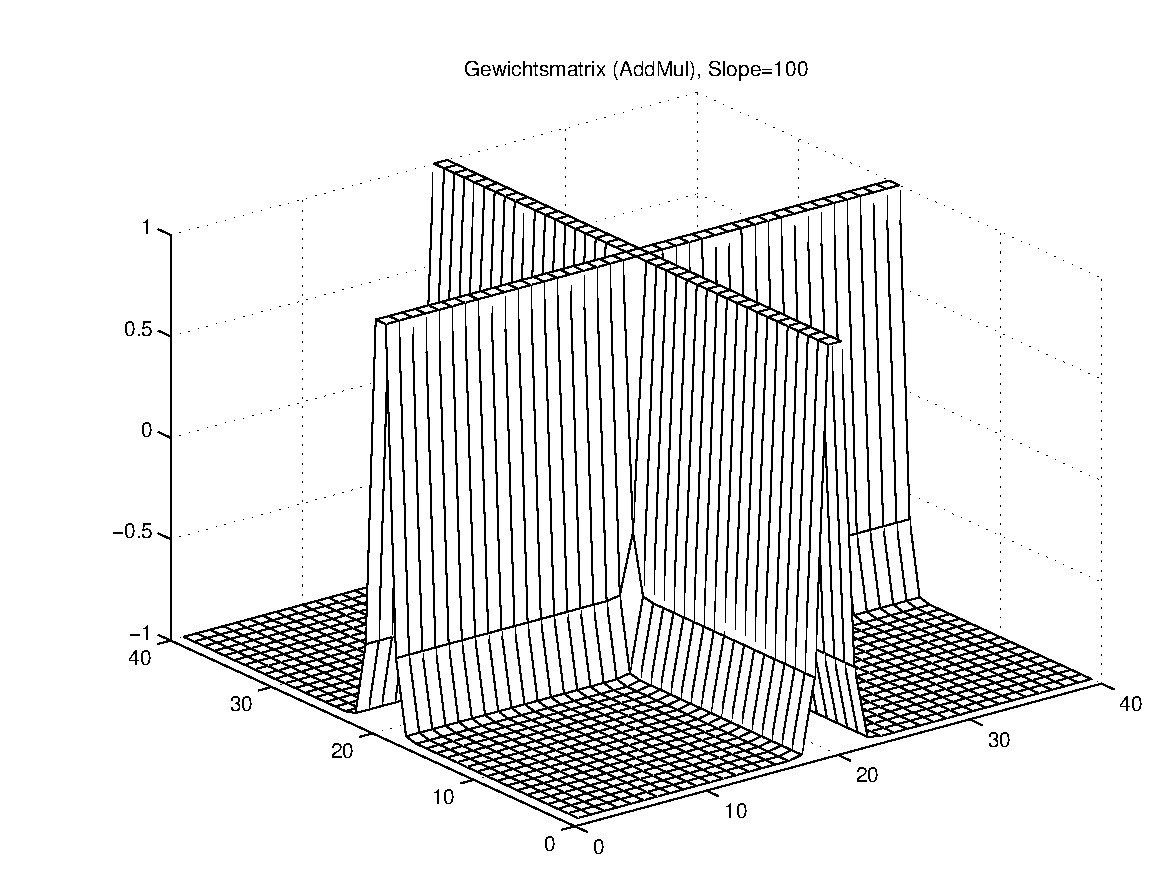
\includegraphics[trim=70 200 32 242, clip, width=0.45\linewidth]{./Bilder/Auswertung/Gewichtsmatrix/Gewichtsmatrix_AddMul_Slope_100}
	\caption{Additive und Multiplikative Überlagerung mit Slope von 100}
	\label{AddMul100}
\end{figure}

\newpage
\subsection{Spezielle Überlagerung}
Bei der Speziellen Gewichtsmatrix hat der Slope keine Auswirkungen. Das war viel mehr ein Versuch, die Auswirkung von erhöhten Gewichten in den Randbereichen zu untersuchen. Sie wurde empirisch aus den Typen: 'Mul1', 'Mul2' und 'AddMul' ermittelt, siehe Listing \ref{code:Special}.
\lstinputlisting[language=MATLAB, caption=Auszug GetGaussWeights: Spezielle Überlagerung \ref{GetGaussWeights}, label=code:Special, numbers=left, firstline=104, lastline=108, firstnumber=104]{../Tool/GetGaussWeights.m}
\begin{figure}[hbt]
	\begin{minipage}{0.48\textwidth}
		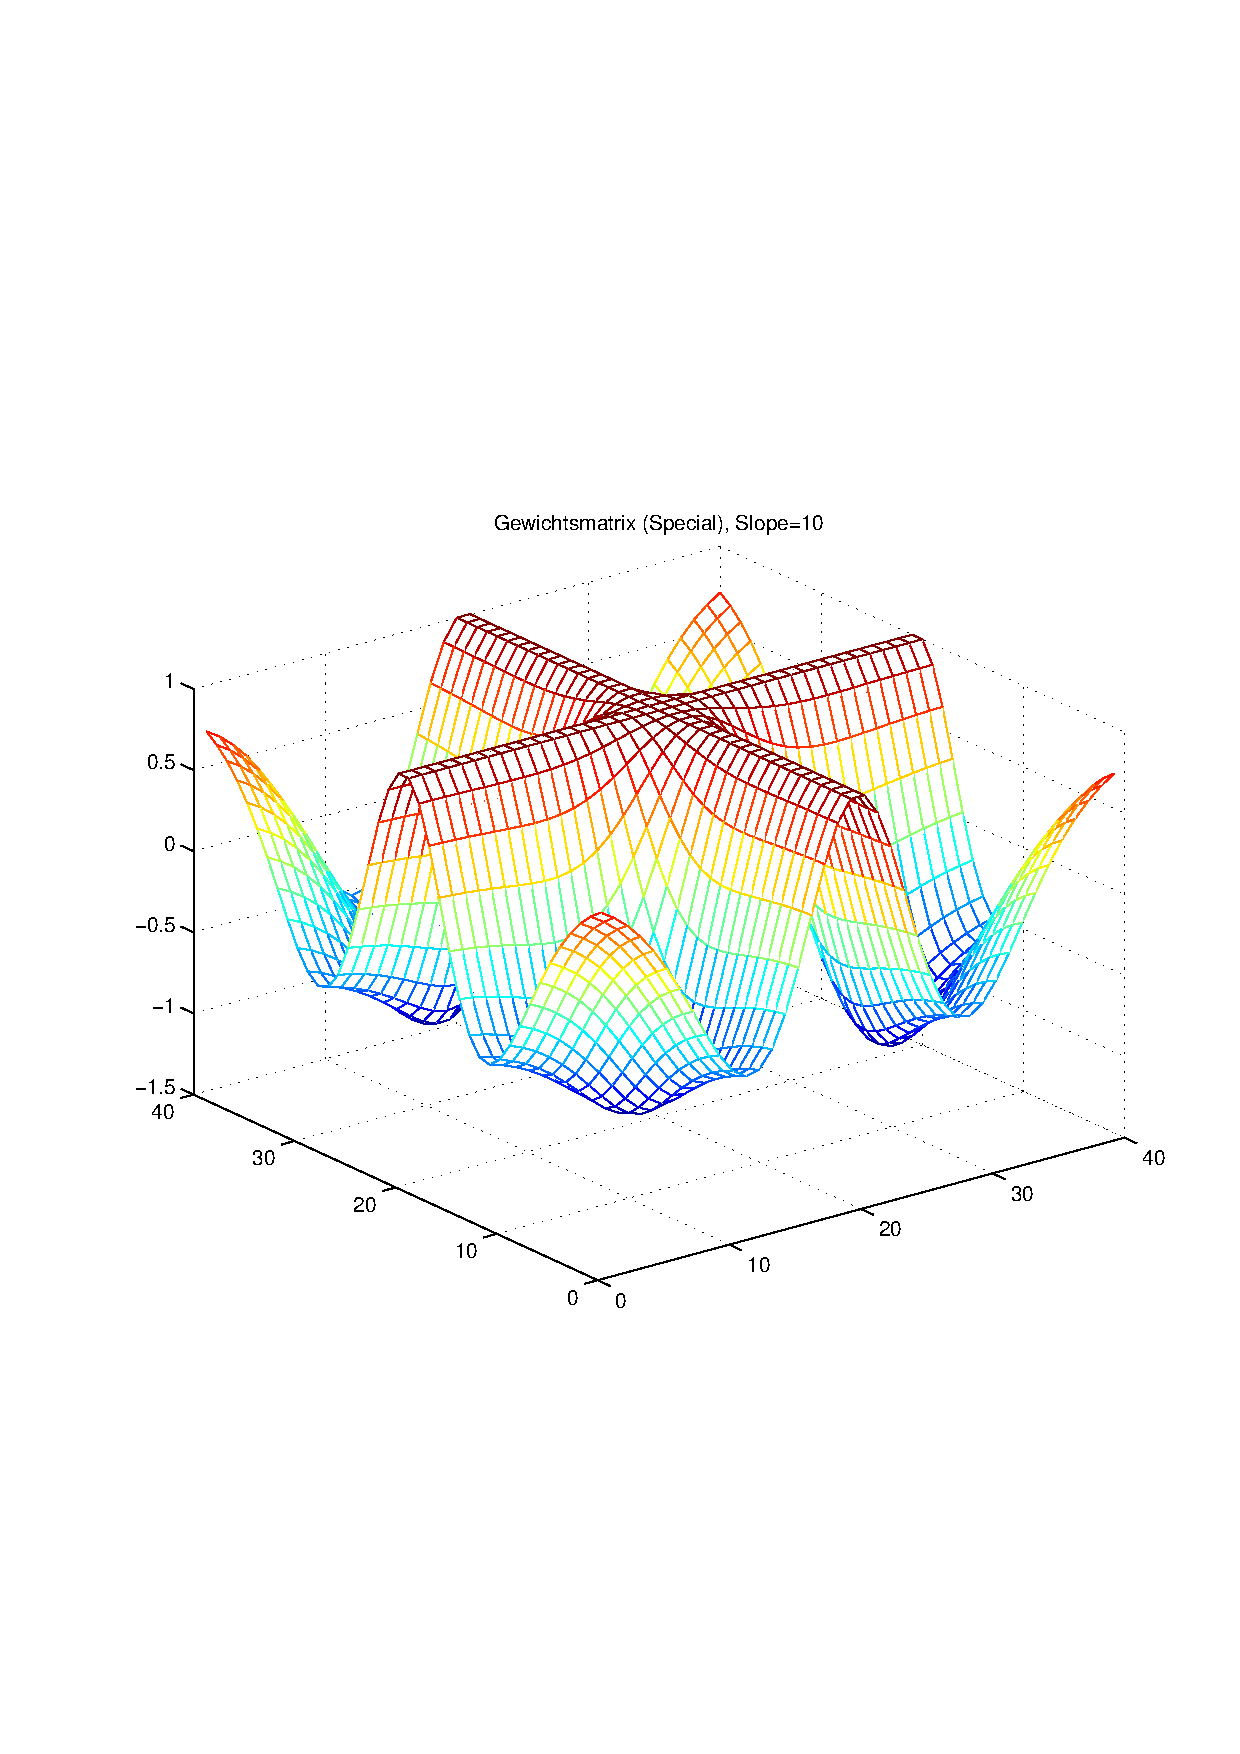
\includegraphics[trim=70 200 32 242, clip, width=\textwidth]{./Bilder/Auswertung/Gewichtsmatrix/Gewichtsmatrix_Special_Slope_10}
		\caption{Spezielle mit Slope 10}
		\label{Spez210}
	\end{minipage}
	\hfill
	\begin{minipage}{0.48\textwidth}
		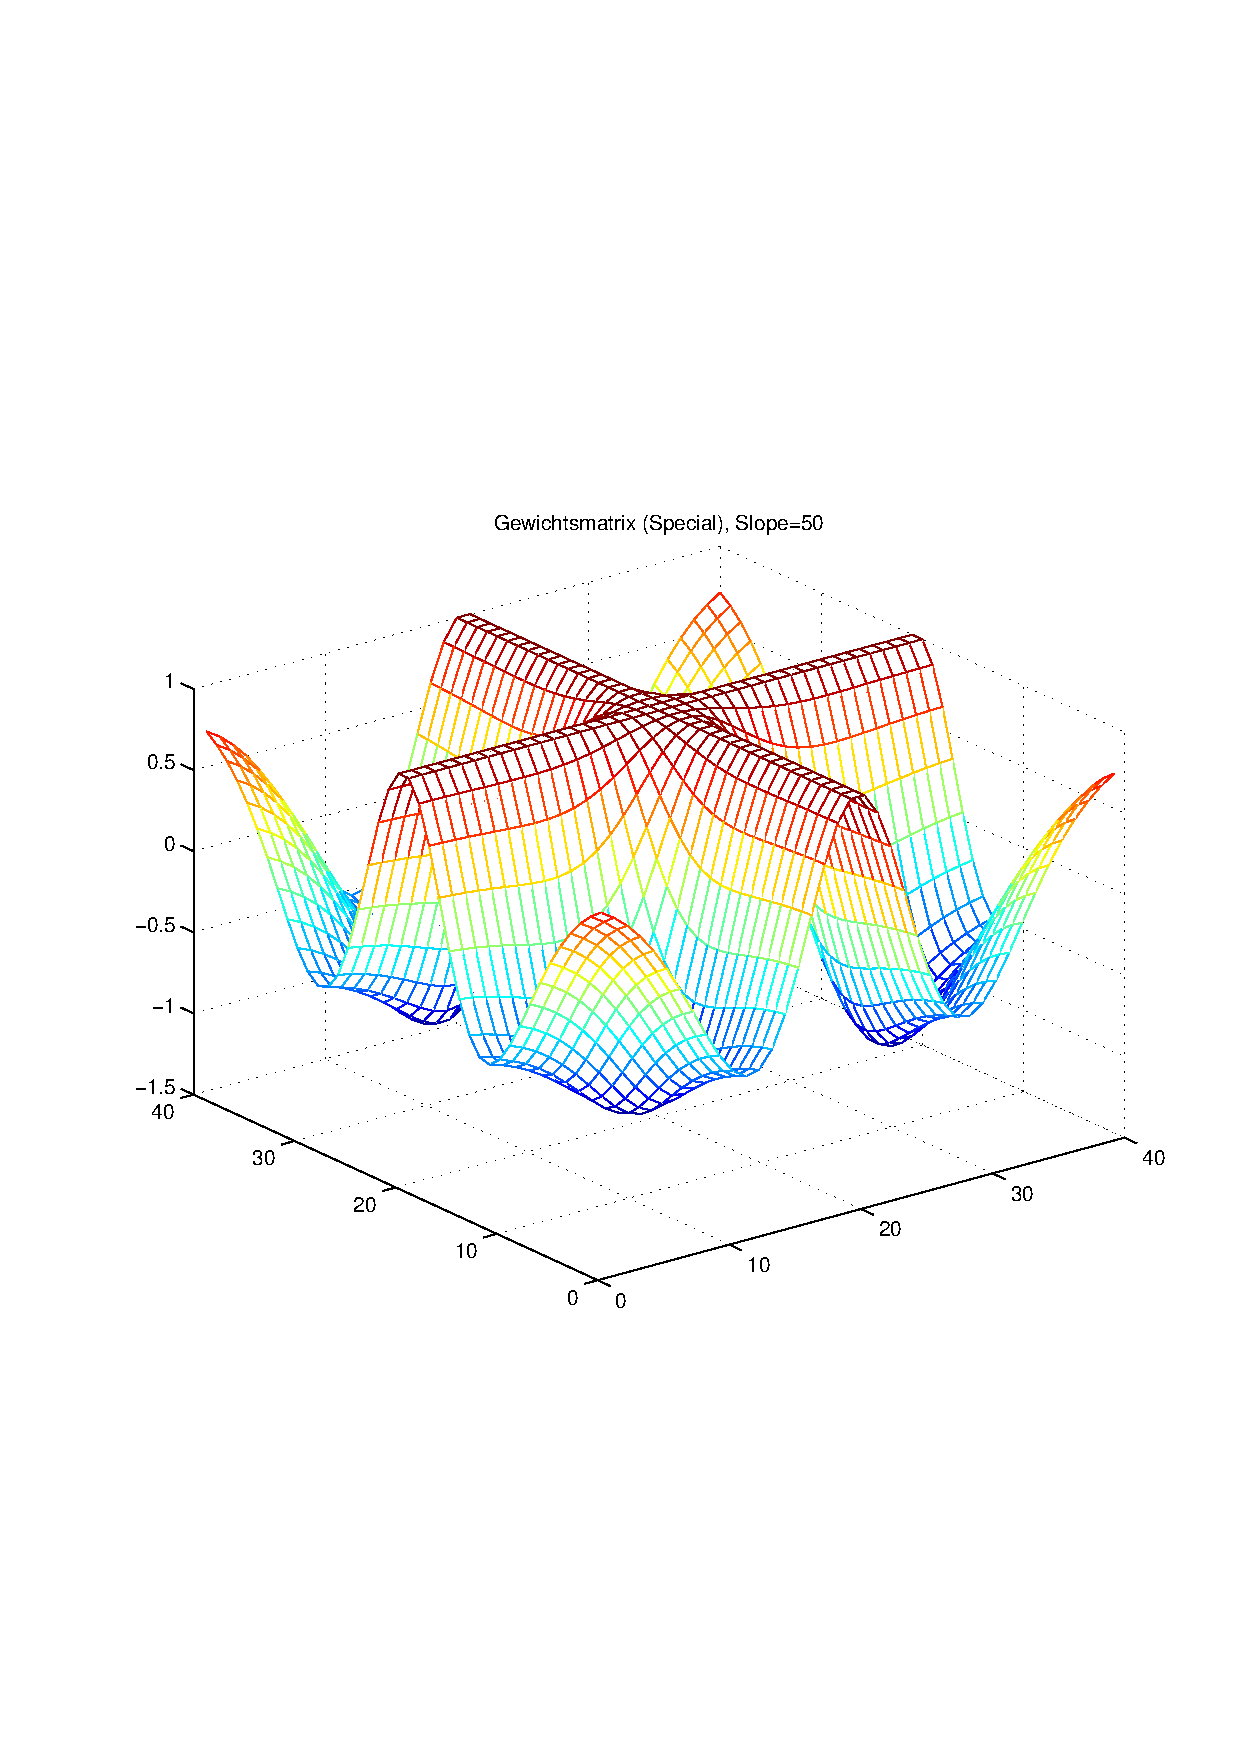
\includegraphics[trim=70 200 32 242, clip, width=\textwidth]{./Bilder/Auswertung/Gewichtsmatrix/Gewichtsmatrix_Special_Slope_50}
		\caption{Spezielle mit Slope 50}
		\label{Spezl50}
	\end{minipage}
\end{figure}
\begin{figure}[hbt]
	\centering
	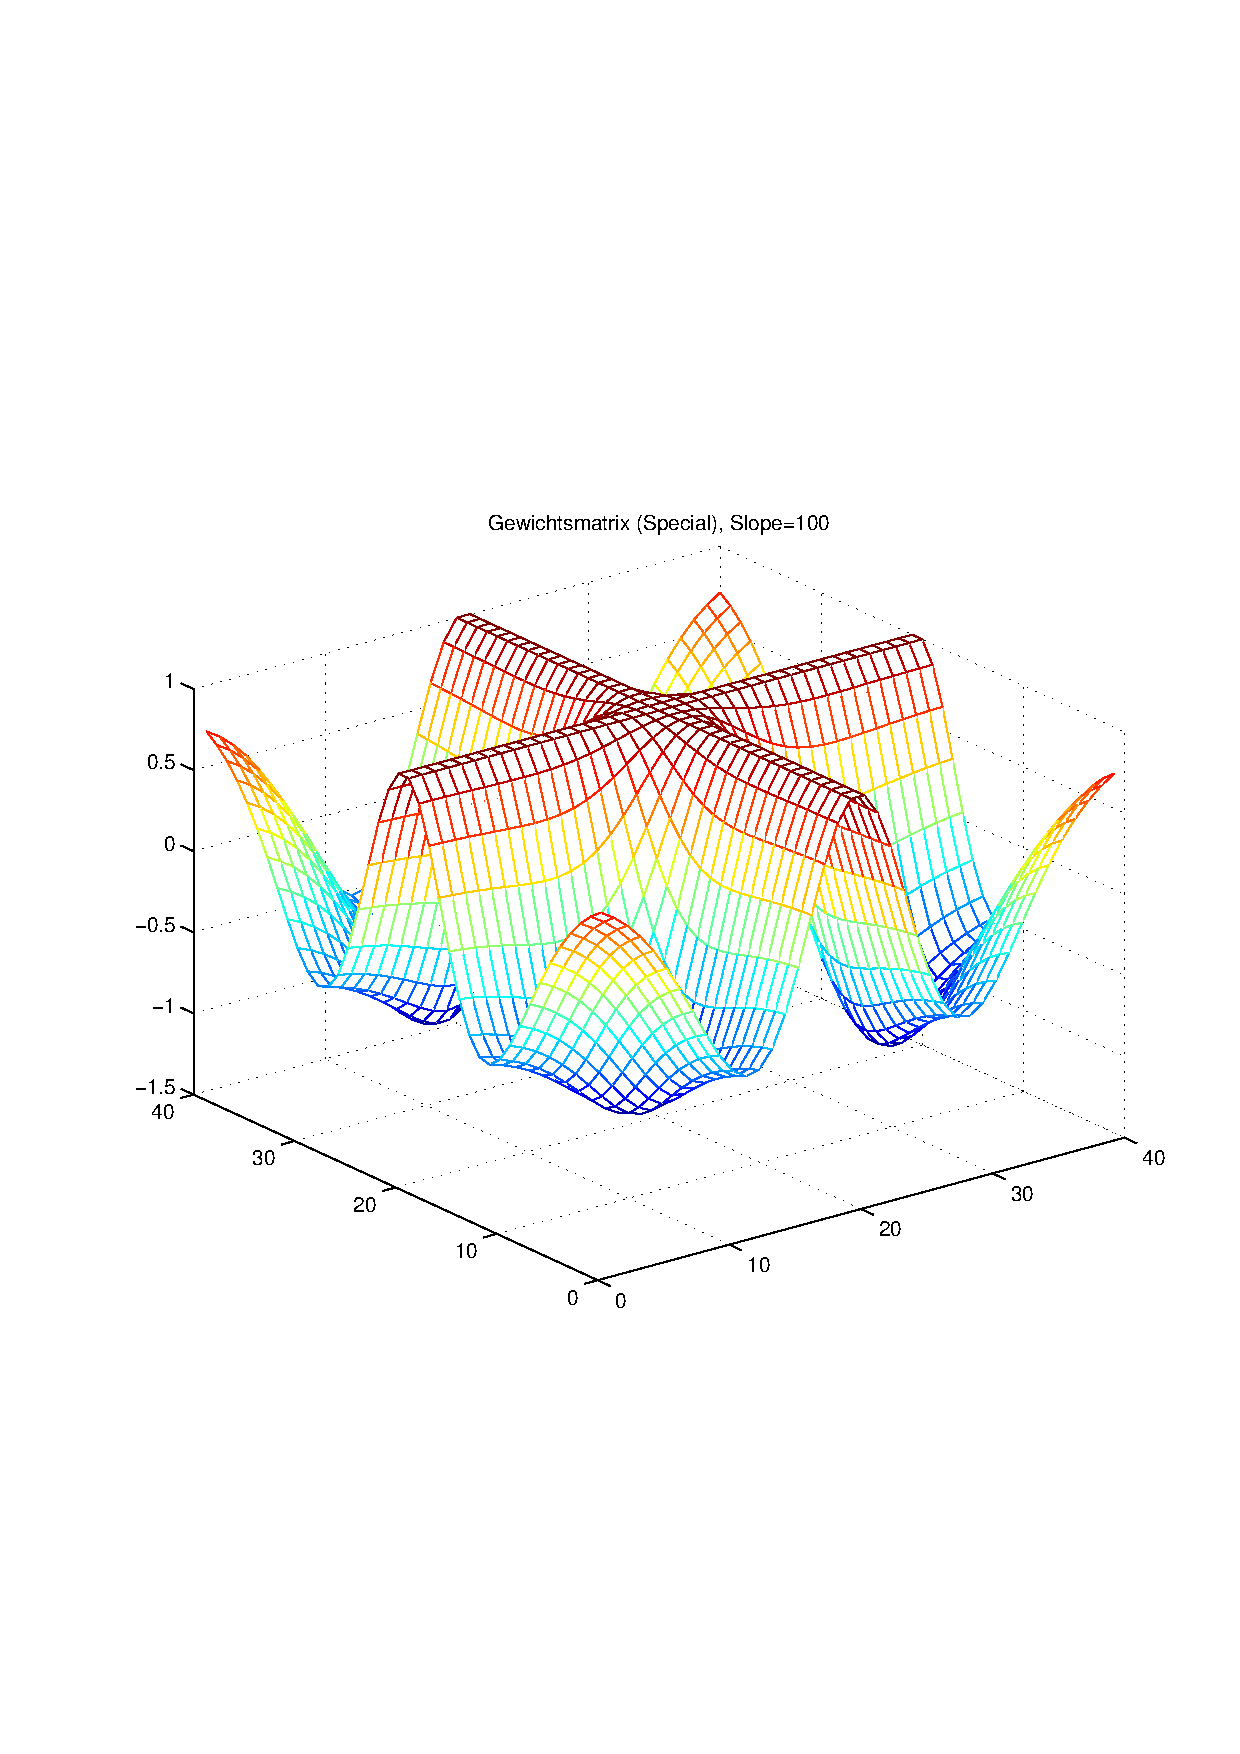
\includegraphics[trim=70 200 32 242, clip, width=0.48\linewidth]{./Bilder/Auswertung/Gewichtsmatrix/Gewichtsmatrix_Special_Slope_100}
	\caption{Spezielle Überlagerung mit Slope von 100}
	\label{Spez100}
\end{figure}